\documentclass[border=6pt]{standalone}
\usepackage[T1]{fontenc}
\usepackage{lmodern}
\usepackage{amssymb}
\usepackage{array}
\usepackage{tikz}
\usetikzlibrary{arrows.meta,calc}
\usepackage{pgfplots}
\pgfplotsset{compat=1.18}
\definecolor{cardblue}{HTML}{114d95}
\definecolor{oldorange}{HTML}{7d1f1b}
\definecolor{aqua}{HTML}{deb520}
\definecolor{notsure}{HTML}{A8A69E}
\newcommand{\pieslice}[4]{%
  \fill[#3, draw=white, line width=1.2pt] (0,0) -- (#1:\R) arc[start angle=#1, end angle=#2, radius=\R] -- cycle;
  \node[font=\small\bfseries, text=white] at ({(#1+#2)/2}:{0.62*\R}) {#4};}
\begin{document}
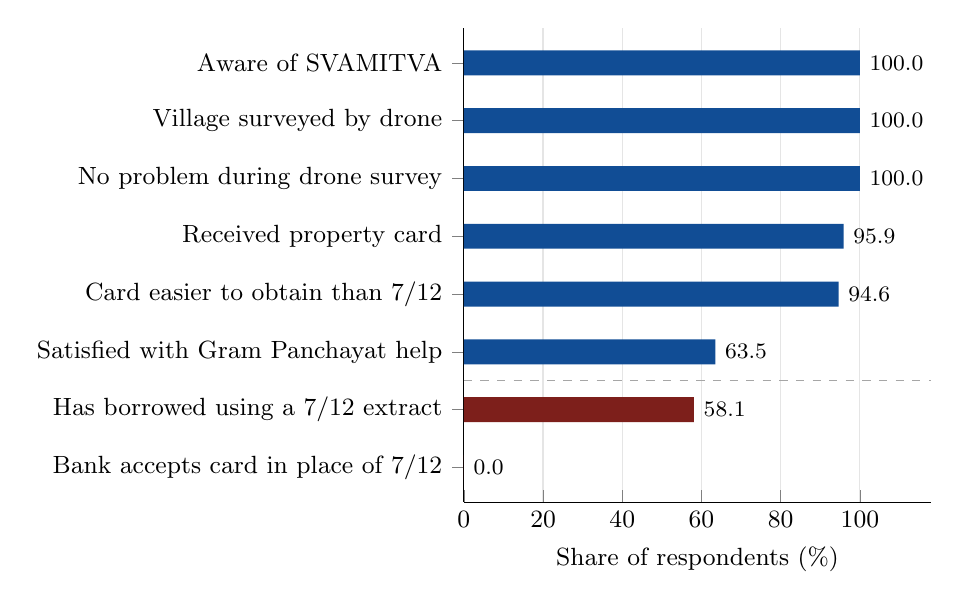
\begin{tikzpicture}
\begin{axis}[
    xbar, bar shift=0pt, bar width=9pt,
    width=0.62\textwidth, height=7.6cm,
    xmin=0, xmax=118, xtick={0,20,40,60,80,100},
    xlabel={Share of respondents (\%)},
    ytick={1,...,8}, y dir=reverse, enlarge y limits={abs=0.6},
    yticklabels={
        Aware of SVAMITVA,
        Village surveyed by drone,
        No problem during drone survey,
        Received property card,
        Card easier to obtain than 7/12,
        Satisfied with Gram Panchayat help,
        Has borrowed using a 7/12 extract,
        Bank accepts card in place of 7/12},
    yticklabel style={font=\small},
    xticklabel style={font=\small}, xlabel style={font=\small},
    axis x line*=bottom, axis y line*=left,
    xmajorgrids, major grid style={draw=black!10},
    nodes near coords, point meta=x,
    nodes near coords style={font=\footnotesize, anchor=west,
        /pgf/number format/.cd, fixed, fixed zerofill, precision=1},
]
\addplot[fill=cardblue, draw=none] coordinates
    {(100,1) (100,2) (100,3) (95.9,4) (94.6,5) (63.5,6)};
\addplot[fill=oldorange, draw=none] coordinates
    {(58.1,7) (0,8)};
\draw[black!35, dashed] (axis cs:0,6.5) -- (axis cs:118,6.5);
\end{axis}
\end{tikzpicture}
\end{document}
